\chapter{Architecture \& Development}
This chapter will go into detail of the development stages of this project, discussing the various decisions, challenges and problems faced during the development of each individual component in the system, and how they were resolved.

\section{System Overview}
The system is separated into two individual development projects, \emph{the web server} which contains the website, game engine and editor, and \emph{the storage server}. These are both web based applications which host a HTTP server through the Python-based Flask microframework. An overview of the system is shown in Figure \ref{fig:overallarchitecture}, which labels the key components of the system in red.

\begin{figure}[h]
	\centering
	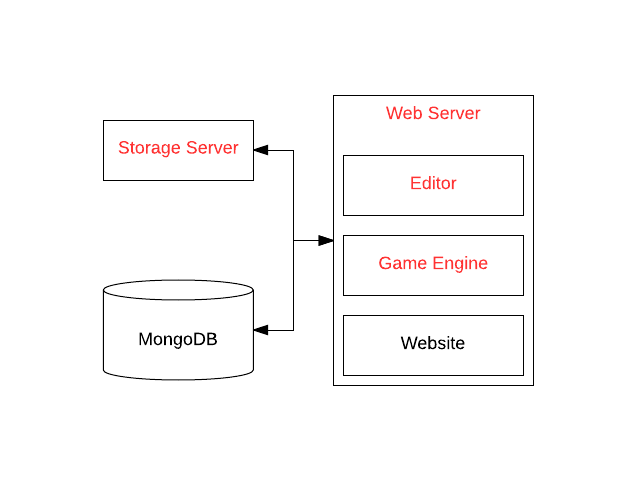
\includegraphics[scale=0.8]{overallarchitecture}
	\caption{Key components in the system}
	\label{fig:overallarchitecture}
\end{figure}

\paragraph{Architectural Patterns.}
The majority of the system follows the MVC (Model-View-Controller) software architectural pattern where possible. This pattern simplifies the development of complex systems by separating the data, display and logic sections into more managable subsystems - the model, view and controller respectively. The structure and architectural pattern of each individual component in this system will be described in-depth in Section \ref{section:systemcomponents}.

% ref MVC, simplifies

\section{Development Environment}
The environment used throughout development of the project consisted of the Sublime Text 3 editor running on the Fedora 19 operating system. For each individual Flask project (The web server and storage server) a virtual environment was set up using \textbf{virtualenv}. Use of virtualenv allowed Python 3.4.2 (separate to the version on Fedora 19) and the required Python libraries to be installed individually for each project.

For both projects, Flask and it's dependencies (itsdangerous, Jinja2, MarkupSafe and Werkzeug) were installed using \textbf{pip} in the virtualenv, along with the libraries specific to each project as seen below:

\begin{itemize}
	\item Web server:
	\begin{itemize}
		\item Flask-Compress
		\item PyMongo
	\end{itemize}
	\item Storage server:
	\begin{itemize}
		\item GitPython and dependencies (gitdb, smmap)
	\end{itemize}
\end{itemize}

The tools required to manage the Amazon Web Services were also installed in this environment, including the AWS CLI (Command Line Interface), and the Elastic Beanstalk CLI. These tools allow remote management of all AWS resources and quick deployment of applications to the Elastic Beanstalk platform.

The Git version control system was used to manage the project in this environment, with the project repository being hosted on GitHub as an external backup source. Originally, the two projects were in the same Git repository, however this proved to be unsuitable as rolling back changes on one project would be troublesome. The two projects were split into their own Git repositories using the \textbf{git subtree split} command, which maintained all commit history relevant to each project.

\section{System Components}
\label{section:systemcomponents}
	\subsection{Web Server}
	The web server is the core part of the system, where all user requests are handled. Everything the user does on the system goes through the web server, so it must be able to handle a lot of users. For this reason the lightweight `microframework' \emph{Flask} was chosen as the base of the server. %todo more

	\subsubsection{Architectural Pattern.}
	The Flask application created for the web server uses a software architectural pattern \emph{similar} to the MVC pattern. Flask lends itself well to the MVC pattern; as each page has it's own URL route (\textbf{Controller}) and template (\textbf{View}), with the route generally populating the template with data (\textbf{Model}). This can be seen visualised in Figure \ref{fig:flaskprocess} which demonstrates how a request is handled by Flask. A client sends a request to the route, the route then retrieves any requested data (Such as a list of published games), then it renders the template for that route with the data. The generated HTML from the template is sent back as the HTTP response.

	\begin{figure}[h]
		\centering
		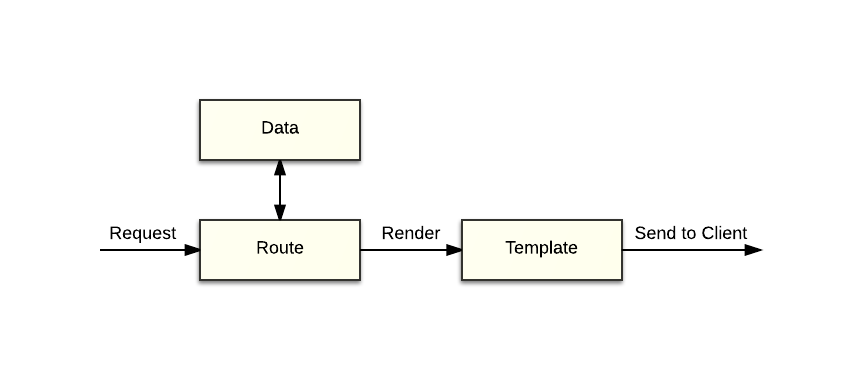
\includegraphics[scale=0.8]{flaskprocess}
		\caption{The Flask request process}
		\label{fig:flaskprocess}
	\end{figure}

	\subsubsection{GitHub API Class}
	A \emph{GitHub} class was created to simplify communication with the GitHub API, by defining methods that would initiate the HTTP connection to GitHub and perform the desired API action, rather than having to set up a connection each time it was needed. Methods were created to handle OAuth operations like obtaining an access token and retrieving user information, as well as getting a list of the user's repositories or creating a new repository on GitHub.

	\subsubsection{Storage API Class}
	The \emph{Storage} class was also created to handle connections to the storage server through it's REST API. A method was created for nearly every route and request type on the storage server, which provided a very simple method of interacting with it from the web application. More information about the routes of the storage server are in section \ref{subsection:devstorageserver}.

	\subsubsection{Configuration}
	The web application loads it's configuration from the config.cfg file in the same directory. The configuration holds the required keys for the GitHub API such as the client ID, client secret and scopes, as well as the storage server's address and port, the MongoDB server address, and the expiry time for the access tokens. These configuration details are loaded in using Flask's built-in config loading methods, and allow the application to be easily reconfigured without having to change any internal code. This was especially useful for deployment, as the address of the storage server and MongoDB server are different once deployed to AWS.

	\subsubsection{Templates.}
	HTML templates are used to render the pages the server sends to the client. These are created using the Jinja2 templating language which is similar to embedding Python in HTML. Jinja2 has the feature of allowing templates to \emph{extend} or \emph{include} other templates, this means that they can be built upon eachother so very little HTML is repeated throughout the files. 

	The template structure used for this website is built by extending a `base' template, which makes the creation of a consistently designed website easy. The base template creates the `html', `head' and `body' tags, links the stylesheets, adds a footer, then includes the `nav' template which has the top bar containing links to all of pages on the website. The rest of the body of the base template is defined as an empty `block'; which can be redefined by a template extending the base (Seen below).
	\lstset{language=HTML,frame=single}
	\begin{lstlisting}

	\end{lstlisting}

	The nav template uses conditionals in Jinja2 to programmatically change how the navigation bar is displayed to the user; it does this by accessing the session variable on the server to check if the user has logged in. When a user is logged in, they are shown the link to the dashboard, along with their avatar, name and a `log out' button. If a user isn't logged in then the `log in' button is shown. This can be seen below:

	\begin{lstlisting}

	<div class="userbox">
	<img src="{{session['user_info']['avatar_url']}}&amp;s=30" alt="">
	{{ session['user_info']['name'] }} 
	<a href="/logout">logout</a>
	</div>

	<form 
		action="https://github.com/login/oauth/authorize" method="get">
		<button type="submit" class="btn btn-default">
			Log in with GitHub
		</button>
		<input type="hidden" name="scope" value="{{config.GITHUB_SCOPES}}"/>
		<input type="hidden" name="client_id" value="{{config.GITHUB_CLIENT_ID}}"/>
	</form>

	\end{lstlisting}

	\subsubsection{Routes}
	The development of this part of the system consisted of developing each URL that users could access on the website. These took the form as routes in the Flask application, designated with a URL containing variables (Denoted with <>), along with HTML templates that get rendered with data from the server (However not every route has a template).

	There is also a global `before\_request' method that is executed just before every request received, which sets up the connection to the MongoDB server, initialises the GitHub API class with the API keys, and set up the storage class that handles connections to the storage server. This simplified using these systems in the routes, as they could be accessed through the \textbf{g} (global) variable in Flask without needing to be set up each time.

	\subsubsection{/}
	The \textbf{/} route is the homepage of the website, which displays some information about Stratus and a short list of published games. This is achieved by getting the list of published games on Mongo, limited to 5 results and sorted by timestamp. The data retrieved is then rendered with the `index.html' template, which loops through the list of games and displays them in div tags with a `play' button linking to the \textbf{/game/<user>/<repo>} route.
	
	\subsubsection{/games}
	The \textbf{/games} route has a similar function to the \textbf{/} route. Instead of listing the most recently published 5 games, it shows an entire list of games published, which is sorted by user and repository.

	\subsubsection{/game/<user>/<repo>}
	The /game route is what users visit when they go to play a game on Stratus. Games that have been published can be accessed by anyone, however if they haven't been published they can only be accessed by the original owner. This is implemented by first checking the Mongo database to see if the game is published; if not then the user's session details are compared to the author of the game. If there are no session details or they don't match, the server will return a `403 Forbidden' page.

	When it has been determined that the user is allowed to play the game, the gamedata JSON and component scripts are retrieved from the storage server. These are then inserted into the `game.html' template, rendering them all in script tags. Component scripts are each given their own script tag by looping through the list of components, and the gamedata is given a script tag with the MIME type `application/json' to make sure it doesn't get executed as JavaScript.

	Originally this was going to be implemented using AJAX to load all files individually, but that was decided against to keep the response time as low as possible. Using AJAX would have also required the implementation of a loading screen to keep the user informed about what was going on.

	A separate template, `engine.html` is also inserted into the game template, which contains all the necessary script files for running a game. This includes the Three.js and Ammo.js libraries, along with all of the Game Engine scripts. This was separated from the game template to reuse it in the game editor.

	At the end of the game template, a small script initialises the game engine, which begins loading in the JSON object and building the scene.

	\subsubsection{/login}
	Authentication is performed using the GitHub OAuth API. This works by setting up an `application' in GitHub, and specifying certain `scopes', which give the application permissions related to controlling the user's settings or repositories. For the purpose of this application, the `user' and `repo' scopes were chosen, to allow the retrieval of user information and the creation of new repositories. After the application was set up, GitHub provided a \textbf{Client ID} and \textbf{Client Secret}; these are used to tell the OAuth system what application the client is using.

	To create the login system, a button is added to the website which redirects the user to the GitHub OAuth page, with the client ID and scope sent with them. This URL takes a form such as:

	\begin{lstlisting}
	https://github.com/login/oauth/authorize?scope=user,repo&client_id=170c030cc1ef6a518a8e
	\end{lstlisting}

	Upon authorising the application, GitHub will redirect the user back to the `Authorization callback URL' (the \textbf{/login} route) specified in the application configuration, providing a \emph{code} in the URL which can be used to get an \textbf{access token} for the user.

	\begin{lstlisting}
	/login?code=a9888d90ed2ac97cee5e
	\end{lstlisting}

	When a user is redirected to the \textbf{/login} route with a code from GitHub, the route uses the code to get the user's access token to complete the GitHub OAuth process. This is done by sending the code, the client ID and the client secret to the GitHub API, using the class described above. The URL of this request takes the form of:

	\begin{lstlisting}
	https://github.com/login/oauth/access_token?code=a9888d90ed2ac97cee5e&client_id=170c030cc1ef6a518a8e&client_secret=3oeqft9w9zd536m0oxar
	\end{lstlisting}

	The GitHub API then responds in a JSON format, providing the access token which allows the web application to perform actions on the user's GitHub account. The user's details are retrieved using this access token, which are then stored with the access token in the user's session in Flask, which allows them to be held on to for the duration of the user's stay on the website without any external storage. 

	After the user's details have been retrieved successfully, the \textbf{/login} route redirects them to the \textbf{/dashboard} route, where they can manage their list of games. The session can now be used to determine if a user is logged in by checking if the access token part of the session exists and is valid.

	\subsubsection{/logout}
	When a user wishes to log out of the system, the /logout route clears the session holding their details, then redirects them back to the homepage. Since the session no longer has their details in it, they will be unable to use any of the features that require them until they log back in. The GitHub OAuth system will remember that the user has authenticated using this application before, so if they choose to log in again, they won't need to authorize the application, and will be logged in straight away.

	\subsubsection{/dashboard}
	The dashboard is where a list of the logged in user's projects are displayed, along with their respective Git status, and whether or not they are published. The dashboard route pulls all the information about the user's repositories on the system from the storage server, using the restful API. Then, for each repository it obtains the git status; checking if there are any uncommitted changes in the repository. The list of published games for the current user is also obtained from the MongoDB database. All of this information is pushed into the `dashboard.html' template, which is rendered and displayed to the user. If the \textbf{/dashboard} route is accessed without a user being logged in, a 403 Forbidden error is shown, however this normally shouldn't occur as the dashboard link is hidden for guests.

	There are a number of actions available to the user on the dashboard, related to the management of their game projects on the system. Each of these actions have their own route on the web application prefixed with /dashboard/ which requires a user to be logged in, and redirects back to the dashboard with a message (Action completed, error occured) when completed. These actions are detailed below:

	\paragraph{publish/<repo>.}
	The publish action toggles whether or not the specified repository of the current user is published on the system. It does this by searching the database to see if it currently is published; if so it deletes the entry in the database. If it isn't published, then it will add an entry specifying the current time as the publishing date.

	There are two problems with this, the first being if the user has another dashboard tab open that hasn't been refreshed, they may end up attempting to publish a game that has already been published in the other tab, causing it to be unpublished. The second problem is that when the game is unpublished and re-published successively the timestamp will update, which could be used to game the system and keep that user's game at the top of the `latest' list.

	\paragraph{init/<repo>.}
	The init action creates a new repository for a game on both the storage server and the GitHub account of the user. A popup on the dashboard asks what the user would like to call their repo, then redirects them to this route. The repository is created by first checking if there is a repository with this name, and aborting the process with a message to the user if that is the case. The route then uses the storage API to create the new repository on the storage server, passing in the user's GitHub access token which is used to complete any git push or pull actions later on. The remote repository on GitHub is created through the GitHub API which is necessary to allow the user to push their changes to GitHub. The new repository is initialised with an empty `gamedata.json' file to signify that it is a Stratus game.

	Any errors that occur during this process will cause the route to redirect back to the dashboard with an error message, explaining what happened to the user. If the process completed successfully, the user is shown a `success' message on the dashboard.

	\paragraph{delete/<repo>.}
	The delete action will delete the specified repository and all changes from the storage server, but not the remote GitHub repo. This is performed through the storage API and discards any changes that weren't pushed to GitHub, which could be devastating to a user if done by accident. The dashboard makes this slightly safer by displaying a popup to the user asking if they really want to delete it before sending them to this route. Any repo that is currently published when being deleted will have their entry removed from the MongoDB \emph{published} collection.

	\paragraph{commit/<repo>.}
	The commit action will create a new commit of any new changes in the specified repository. The dashboard provides a pop-up textarea for inputting the commit message, which then POSTs the message to the repository specific route when the user submits it. 

	The commit is made through the storage API, by first retrieving the status of the repository; which contains a list of modified, deleted or untracked files. This list is sent along with the commit message to the storage server, which performs the \textbf{git add} and \textbf{git remove} operations then creates the commit with the message.

	One problem that was encountered while developing this route was that any commit that was pushed to GitHub didn't show the correct author. This was resolved by sending along the user's name and email address from the session to the storage server, which then added those to the commit as the `committer'.

	\paragraph{push/<repo>.}
	The push route instructs the storage server to push any commits that have been made to the GitHub remote server. There is a possibility for the user to encounter an error here if they have been changing the repository outside of Stratus; that is if the remote server (GitHub) has changes that are ahead of the repository on the storage server. If a user attempts to push when this is the case, GitHub will reject the push.

	In the event that this happens, the user will receive a message suggesting that they attempt to pull the remote changes before pushing. This will most likely resolve the issue, as the changes from the remote and local changes will be merged automatically on the storage server. The changes can then be pushed as normal.

	\paragraph{pull/<repo>.}
	The pull route is used to retrieve any changes from the remote git server, GitHub. This is completed by contacting the storage server through the API and telling it to perform the git pull operation on the specified repository. As above, there are some issues that may be run into with this, specifically related to \textbf{merge conflicts}.

	Merge conflicts occur when remote changes are unable to be merged automatically with the local changes of a repo during a pull. In this situation, the file(s) that have conflicting data must be manually patched, as the lines will be replaced with \textbf{both} sets of conflicting data. An example of what this looks like is below:

	\begin{lstlisting}
"scale": {
        "type": "vector",
        "parameters": [
<<<<<<< HEAD
                110.57,
                106.95,
                16.31
=======
                1000,
                800,
                1
>>>>>>> 96a40b322727f0c034e26a438461d53962bdec7e
        ]
}
	\end{lstlisting}

	When this is the case, it's impossible to create a commit until this has been resolved; as it will always fail. This can also cause the editor and game routes to become dysfunctional if it happens on the gamedata.json file, as it will no longer be valid JSON.

	Currently there is no implemented method to resolve merge conflicts on Stratus, however this is one of the first features that will be added if the project is continued, as it will greatly help with the collaboration of team members working on a game together through Git.

	\paragraph{clone/<repo>.}
	The clone route performs an action similar to the \textbf{git clone} command. It \emph{clones} the specified remote repository from GitHub, along with all of it's contents, and stores them on the storage server. This is actually done as a two step process, where the local repository is initialised with the same details as the remote repository, then it is \emph{pulled} to retrieve all of the contents from the remote. A list of repositories on GitHub is retrieved using the GitHub API and displayed on the dashboard, which allows the user to select from a list rather than having to input the repository name.
	
	\subsubsection{/editor/<repo>}
	The editor route is where users will be able to modify their games. Users may click on the `edit' button for one of their games in the dashboard, which will bring them to the editor for their selected game. In a similar method to the \textbf{/game/<user>/<repo>} route, all of the game files are retrieved from the storage server and then inserted into the `editor.html' template, along with the list of files in the repository. The template itself loads all of the necessary files for the editor, such as the numerous `view' script files, and the templates for those views. This is discussed further in section \ref{subsection:gameeditor}.

	Since the editor is designed to modify files for the user, it needed a method of storing and retrieving the files on the storage server. This was provided by the \textbf{/editor/<repo>/<file>} route. This route accepts GET, POST and DELETE requests in a similar manner to the RESTful API on the storage server, in order to update files such as the gamedata.json file, or custom component scripts. This was needed as there is no way for the client to communicate with the storage server directly.

	\subsection{Storage Server}
	\label{subsection:devstorageserver}

	The storage server is a REST API that provides a central access point for each web server instance's storage needs. It was required to be separated from the web server so that the stored data would be persistent accross each instance of the web server that is created. A REST (Representational State Transfer) API was chosen for this part of the server as it provides a very simple interface for the management of resources; in this case it is for managing files on the filesystem. 

	The storage API is developed using Flask and provides several routes (URLs) that are prefixed with a user and repository for specifying the game to work on. These routes usually take the form of `/<user>/<repo>/<action>/<...>', with a good example being `/dcrn/stratus-pool/file/gamedata.json'. Each route supports several HTTP request types, including \textbf{GET}, \textbf{POST}, \textbf{PUT} and \textbf{DELETE}; with each request type having an action to perform on the resource requested:
	\\
	~\\
	GET requests will \textbf{retrieve} a resource, or the status of a resource.\\
	POST requests will \textbf{create} a resource or perform an action.\\
	PUT requests will \textbf{update} a resource.\\
	DELETE requests will \textbf{delete} a resource.\\

	\subsubsection{Architectural Pattern.}
	The software pattern used for the storage server is similar to the MVC system generally used in Flask, however MVC is more suited towards applications that have a user interface; a `view'. In this case the JSON output by the RESTful API could be considered the view, with the controller being routes and the model being the file structures.

	\subsubsection{GitPython}
	The GitPython library was included in this project to provide a method of performing git operations on the local files via Python. GitPython is a wrapper around the \textbf{git} command, which provides an interface that is familiar to executing git commands manually. The usage of this library is seen below in the routes related to performing Git operations.

	% todo ref gitpython, ref api?

	\subsubsection{Routes}

	GET - Retrieve information:
	
	\paragraph{/<user>.}
	This route retrieves the list of repositories on the storage server for the specified user; obtained by searching the user's directory with Python's built-in \textbf{os.listdirs} function. For each directory found, it checks if there is a git repository initialised; by using the GitPython library's git.Repo method. The git.Repo method will throw an InvalidGitRepositoryError exception if the directory has no git repository in it.

	Then, for each repository, the number of \emph{unpushed commits} is calculated to provide the dashboard with information about the remote git repository. This is done by calling repo.iter\_commits, a method similar to the \textbf{git rev-parse} command. Iter\_commits is used to retrieve the symmetric difference between the last pulled remote version and the latest commit (the HEAD) by specifying the git rev-parse arguments `remote/branch..' which is a shorthand version of `remote/branch..HEAD'. This only works if there \textbf{is} a remote version at all, which is troublesome in the case of newly created repositories. Because of this, the remote reference is checked to see if it exists, and if it doesn't then the number of commits ahead of the remote is set to 1.

	The output of this route is returned as a JSON object listing the repository names as the keys and their values being the number of commits ahead of the remote (Seen below). In the event of an error, an empty JSON object is returned and the appropriate status code is returned; such as 404 for a user that doesn't exist.

	\begin{lstlisting}
{
	"stratus-pool": 0,
	"test-repo": 0,
	"test-repo2": 1
}\end{lstlisting}

	\paragraph{/<user>/<repo>/status.}
	The status route retrieves the status of a git repository, similar to the \textbf{git status} command, returning a list of added, deleted, modified, renamed and untracked files in the specified repository. The GitPython library is used to obtain the most recent commit (if any), and compares it to the working version of the repository, calculating the `diffs' (differences) between them. The diffs are then iterated, categorising the changes by type (modified, deleted, ..) and storing the filenames for that diff. The results of this are then sent back in a JSON format along with a list of any untracked files in the repository. In the case that there is no previous commit to compare to, only the list of untracked files in the repository is used.

	\paragraph{/<user>/<repo>/tree/<path>.}
	The tree route uses the built-in Python function \textbf{os.walk} to get the directory tree of all files in the specified repository and path. This is used in the editor when listing out the custom components users have made. The `path' specified at the end of the route is optional, and defaults to the root of the repository. The result of this is returned in a JSON format, which structures directories as an \textbf{object} and files as the value \textbf{true} (Seen below).

	\begin{lstlisting}
{
	"components": {
		"cuecontroller.js": true
	},
	"gamedata.json": true
}\end{lstlisting}
	
	POST - Perform action:

	\paragraph{/<user>/<repo>/push/<remote>.}
	The push route performs the \textbf{git push} action on the repository, with the specified remote. This is equivalent to running `git push <remote> master' in a terminal. This is done by finding the remote on the repo object (if it exists), then running the GitPython method \textbf{remote.push}, specifying the a reference to the latest commit in the repo (repo.head.reference). If the push command is rejected by the remote for some reason, the output from this route will be a 409 Conflict status code, along with an empty JSON object. If the push is completed successfully, a 200 OK status code is returned.

	\paragraph{/<user>/<repo>/pull/<remote>.}
	The pull route performs a \textbf{git pull} action using GitPython. This is done by first fetching any changes from the remote using the remote.fetch method, which is similar to the \textbf{git fetch} action, then replacing the local HEAD reference with the remote HEAD reference using the remote.pull method. When the pull action is completed, the route returns an empty JSON object and the 200 OK status code. If fetching or pulling the changes causes any errors, this will return a 409 Conflict status code.

	\paragraph{/<user>/<repo>/commit.}
	This route is used to create a commit on the storage server, and is similar to using the \textbf{git add}, \textbf{git remove} and \textbf{git commit} commands all together. The route requires that some JSON is sent along with the POST request, which should contain a list of files to be added and removed, and a commit message.

	The list of files to be added is iterated and added to the repository's index (Also referred to as the staging area), which is a list of files that will be in the next commit. Any files that are in the removal list are removed from the index. When this is completed, a new commit is created, specifying the message passed in with the JSON. This will automatically push the new commit to the HEAD reference.

	An issue that was encountered here was that when the commits were pushed to GitHub, it showed them as being made by `root', instead of the correct author. This was resolved by sending the author details (full name, email address) over from the web application, and setting them as the author and committer on the commit.
	
	GET/PUT/POST/DELETE - Control resource:
	
	\paragraph{/<user>/<repo>.}
	\paragraph{/<user>/<repo>/file/<path>.}

	% - Pattern - MVC-like
	% - restful API, flask app
		% - GitPython usage
		% - git operations, access_token, remotes
	% - Talk about each API route individually
	% Config files

	% - mongodb
	\subsection{Game Engine}
	% - ECS pattern
	% - "Game" object.
	% - Loading from JSON, initialization
	% - Walkthrough of how the process works. Setting up renderer in Game, updating all scenes with deltatime, updating all entities, updating all components.
	% - Adding, removing components
	% - Using Three.js - setting up the renderer, setting up the Scene to add threeobjs as they are added
	% - Using Ammo.js - Setting up the world, gravity etc, adding ammoobjs as they are added
	% - Simplifying the two libraries into the ECS architecture, predefined components
	% 	This was achieved by etc.
	% - Each pre-defined component
	\subsection{Game Editor}
	\label{subsection:gameeditor}
	% - Pseudo MVC microframework
		% Looked at frameworks, all too heavy
		% Just made my own to keep it simple, based on something similar to backbone
	% - Detail each view
	% - Scene view - 
			% How it loads the gamedata, selection object
	% - Tying in the game engine with the storage backend
	% - Properties of both the gamedata json and the displayed game entities
	% - Scripts, Ace editor
	% - autosaving
	\subsection{Scalable Cloud Deployment}
	% - Setting up AWS
	% - Load balancing, separating web from storage
	% - SSH, Git, tools
	% - Deploying to Elastic Beanstalk {eb cli}
	% - Storage server {Setting up MongoDB, git, cloning the storage repo}
		% - Deployment was difficult compared to Elastic Beanstalk (used git to deploy latest version)

\section{Deployment to AWS}
% How everything was deployed etc

\section{Key Development Components}
% Identify key development components
% Key components were the game engine, editor, web server (load balancing) and storage.
% Git integration wasn't as important to functionality

\section{External APIs}
% Indentification/explanation of external APIs used vs own code. 

\section{List of Classes}
% List of classes of your code
% Write block comments for code during this process?